\documentclass[tikz,border=12pt]{standalone}
\usepackage[T1]{fontenc}
\usepackage{mathpazo}
\usepackage{amsmath,amssymb}
\usetikzlibrary{arrows.meta, calc}

\definecolor{stblue}{HTML}{7B97AD}
\definecolor{rwgold}{HTML}{B8995E}
\definecolor{sage}{HTML}{7A9A7E}
\definecolor{dkbrown}{HTML}{3D3530}
\definecolor{wmgray}{HTML}{7B7067}
\definecolor{cream}{HTML}{F9F6F0}
\definecolor{border}{HTML}{D4C9B8}
\definecolor{terracotta}{HTML}{C47A6A}
\definecolor{lavender}{HTML}{907EA0}

\begin{document}
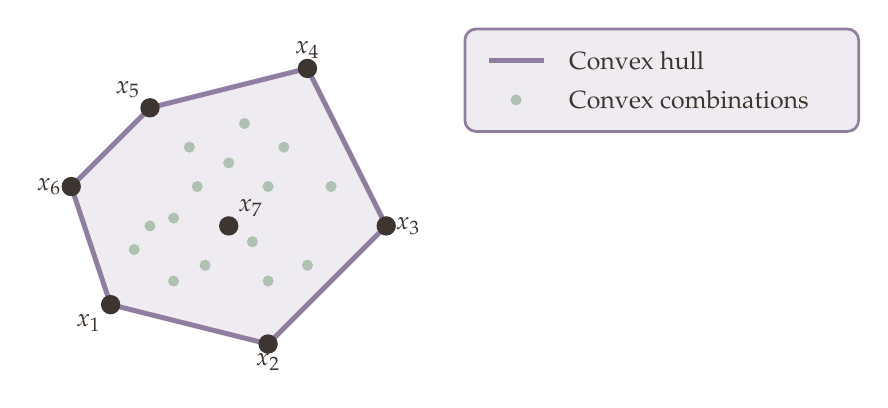
\begin{tikzpicture}

% Points
\coordinate (p1) at (1,1);
\coordinate (p2) at (3,0.5);
\coordinate (p3) at (4.5,2);
\coordinate (p4) at (3.5,4);
\coordinate (p5) at (1.5,3.5);
\coordinate (p6) at (0.5,2.5);
\coordinate (p7) at (2.5,2);   % interior point

% Convex hull (filled)
\fill[lavender!15] (p6) -- (p1) -- (p2) -- (p3) -- (p4) -- (p5) -- cycle;
\draw[lavender, line width=1.8pt] (p6) -- (p1) -- (p2) -- (p3) -- (p4) -- (p5) -- cycle;

% Interior convex combinations (scatter)
\fill[sage!60] (1.8,2.1) circle (2pt);
\fill[sage!60] (2.2,1.5) circle (2pt);
\fill[sage!60] (3.0,2.5) circle (2pt);
\fill[sage!60] (2.8,1.8) circle (2pt);
\fill[sage!60] (1.5,2.0) circle (2pt);
\fill[sage!60] (3.2,3.0) circle (2pt);
\fill[sage!60] (2.0,3.0) circle (2pt);
\fill[sage!60] (2.5,2.8) circle (2pt);
\fill[sage!60] (1.3,1.7) circle (2pt);
\fill[sage!60] (3.8,2.5) circle (2pt);
\fill[sage!60] (2.1,2.5) circle (2pt);
\fill[sage!60] (3.0,1.3) circle (2pt);
\fill[sage!60] (2.7,3.3) circle (2pt);
\fill[sage!60] (1.8,1.3) circle (2pt);
\fill[sage!60] (3.5,1.5) circle (2pt);

% Original points (on top)
\foreach \p/\lab in {p1/$x_1$, p2/$x_2$, p3/$x_3$, p4/$x_4$, p5/$x_5$, p6/$x_6$, p7/$x_7$} {
  \fill[dkbrown] (\p) circle (3.5pt);
}

% Labels
\node[dkbrown, font=\small, anchor=north east] at (p1) {$x_1$};
\node[dkbrown, font=\small, anchor=north] at (p2) {$x_2$};
\node[dkbrown, font=\small, anchor=west] at (p3) {$x_3$};
\node[dkbrown, font=\small, anchor=south] at (p4) {$x_4$};
\node[dkbrown, font=\small, anchor=south east] at (p5) {$x_5$};
\node[dkbrown, font=\small, anchor=east] at (p6) {$x_6$};
\node[dkbrown, font=\small, anchor=south west] at (p7) {$x_7$};

% Legend
\fill[lavender!15, rounded corners=4pt] (5.5,3.2) rectangle (10.5,4.5);
\draw[lavender, line width=1pt, rounded corners=4pt] (5.5,3.2) rectangle (10.5,4.5);
\draw[lavender, line width=1.8pt] (5.8,4.1) -- (6.5,4.1);
\node[dkbrown, font=\small, anchor=west] at (6.7,4.1) {Convex hull};
\fill[sage!60] (6.15,3.6) circle (2pt);
\node[dkbrown, font=\small, anchor=west] at (6.7,3.6) {Convex combinations};

\end{tikzpicture}
\end{document}
